\documentclass{beamer}
\usetheme{Boadilla}
\usecolortheme{sidebartab}
\beamertemplatenavigationsymbolsempty
\setbeamertemplate{footline}[frame number]
\usepackage{hyperref} 
\usepackage{graphicx}
\usepackage{color}
\usepackage{booktabs}
\usepackage{listings}
\usepackage{soul}
\usepackage{tikz}
\usepackage[utf8]{inputenc}
\usepackage{CJKutf8}
\usepackage[export]{adjustbox}
\usetikzlibrary{shapes.geometric}

\definecolor{gray}{rgb}{0.4,0.4,0.4}
\definecolor{darkblue}{rgb}{0.0,0.0,0.6}
\definecolor{cyan}{rgb}{0.0,0.6,0.6}
\definecolor{lightgray}{gray}{0.8}

\lstset{
	basicstyle=\ttfamily,
	columns=fullflexible,
	showstringspaces=false,
	commentstyle=\color{gray}\upshape
}

\lstdefinelanguage{XML}
{
	morestring=[b]",
	morestring=[s]{>}{<},
	morecomment=[s]{<?}{?>},
	stringstyle=\color{black},
	identifierstyle=\color{darkblue},
	keywordstyle=\color{cyan},
	morekeywords={xmlns,version,type}% list your attributes here
}

\makeatletter
\newcommand\SoulColor{%
	\let\set@color\beamerorig@set@color
	\let\reset@color\beamerorig@reset@color}
\makeatother

\lstset{language=XML}

\title{XML und RDF im Informationsmanagement}
\author{Markus Stocker}
\date{18. Juni 2018}

\begin{document}

\maketitle

\begin{frame}{Rekapitulation}
	
	\begin{itemize}
		\item Was ist eine Ontologie (in der Informatik)
		\item Was sind die wesentlichen Bestandteile einer Ontologie?
		\item Wie ist der Aufbau einer Ontologie (TBox, ABox)
		\item Was ist bei der Entwicklung von Ontologien besonders schwierig?
		\item Welche Wissensquellen gibt es?
		\item Was ist Prot{\'e}g{\'e}?
	\end{itemize}
	
\end{frame}

\begin{frame}{Übersicht}
	
	\begin{itemize}
		\item Informationsmanagement, -infrastruktur, -system
		\item Was ist Information?
		\item XML und RDF: Rollen im Informationsmanagement
		\item Information in Forschungsinfrastrukturen
		\item Und zum Schluss ein Projektvorschlag
	\end{itemize}
	
\end{frame}

\begin{frame}{Informationsmanagement}
	
	\begin{itemize}
		\item Steht für das Verwalten von Information
		\item Planen, Gestalten, Überwachen und Steuern von Information
		\item Versorgung des Unternehmens mit Information
		\item Insb. notwendige Information zur Erreichung strategischer Ziele
		\item Information als ``dritten Produktionsfaktor'' (nach Kapital und Arbeit)
		\item Information als unternehmerische Ressource
		\item Entwickelt und nutzt eine entsprechende Informationsinfrastruktur
	\end{itemize}
	
	\begin{flushright}
		\scriptsize\url{https://de.wikipedia.org/wiki/Informationsmanagement}
	\end{flushright}
	
\end{frame}

\begin{frame}{Informationsinfrastruktur}
	
	\begin{itemize}
		\item Ist eine ``Ermöglichungsstruktur''
		\item Für die Erzeugung, Verarbeitung und Verwendung von Information
		\item Informationsinfrastruktur bietet Basisleistungen
		\item Dient nicht unmittelbar der Produktion
		\item Infrastruktur ist ``unsichtbar'', ``verborgen''
		\item Man bemerkt Infrastruktur nur dann, wenn diese ausfällt
		\item Telefon-, Breitband-, Daten-, Funknetze bilden die Grundlage
		\item Eine Gesamtheit an interdependenten Informationssysteme
	\end{itemize}
	
	\begin{flushright}
		\scriptsize\url{https://de.wikipedia.org/wiki/Informationsinfrastruktur}
	\end{flushright}
	
\end{frame}


\begin{frame}{Informationssystem}
	
	\begin{itemize}
		\item Ein soziotechnisches System (Mensch/Aufgabe/Technik-System)
		\item Deckung der Informationsnachfrage durch Informationsproduktion
		\item Mensch ist der Anwender der Aufgaben erfüllen möchte
		\item Entwickler ebenfalls dem Strukturelement Mensch zugeordnet
		\item Aufgabe ist das Problem, das mit dem System gelöst werden soll
		\item Technik besteht aus der Soft- und Hardware des Systems
		\item Erfüllung Verarbeitung-, Verteilungs- und Speicherungsprozessen
		\item Informationssysteme sind Ressourcen einer Informationsinfrastruktur
	\end{itemize}
	
	\begin{flushright}
		\scriptsize\url{https://de.wikipedia.org/wiki/Informationssystem}
		% Man bezeichnet diese interdependente Gesamtheit als Informationsinfrastruktur
	\end{flushright}
	
\end{frame}

\begin{frame}[plain]{}
	
	\Huge
	\begin{center}
Was ist Information?	
	\end{center}
	
\end{frame}

\begin{frame}{DIKW Modell}
	
	\begin{minipage}[t]{0.65\textwidth}
		\begin{itemize}
			\item Daten: Symbole/Zeichen, keine Bedeutung
			\item Information: Ist nutzbar, bedeutungsvoll
			\item Wissen: Organisierte Information
		\end{itemize}
	\end{minipage}
	\begin{minipage}[t]{0.3\textwidth}
		\begin{figure}
			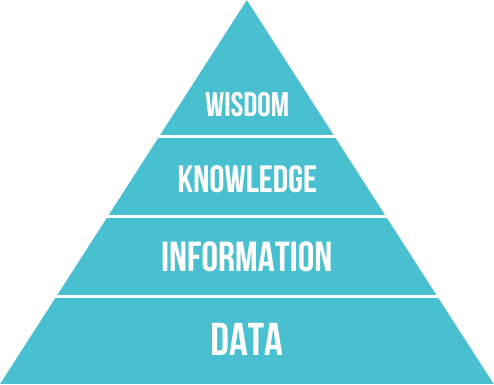
\includegraphics[scale=0.3,right]{dikw-pyramid.png}
		\end{figure}
	\end{minipage}
	
	\tiny
	\begin{flushright}
		Image by Longlivetheux - Own work, CC BY-SA 4.0,\\ \url{https://commons.wikimedia.org/w/index.php?curid=37705247}\\
		
		\vspace{0.2cm}
		\url{https://en.wikipedia.org/wiki/DIKW_pyramid}
	\end{flushright}
	
\end{frame}

\begin{frame}{Von Daten zu Wissen: Prozesse}
	
	\begin{figure}
		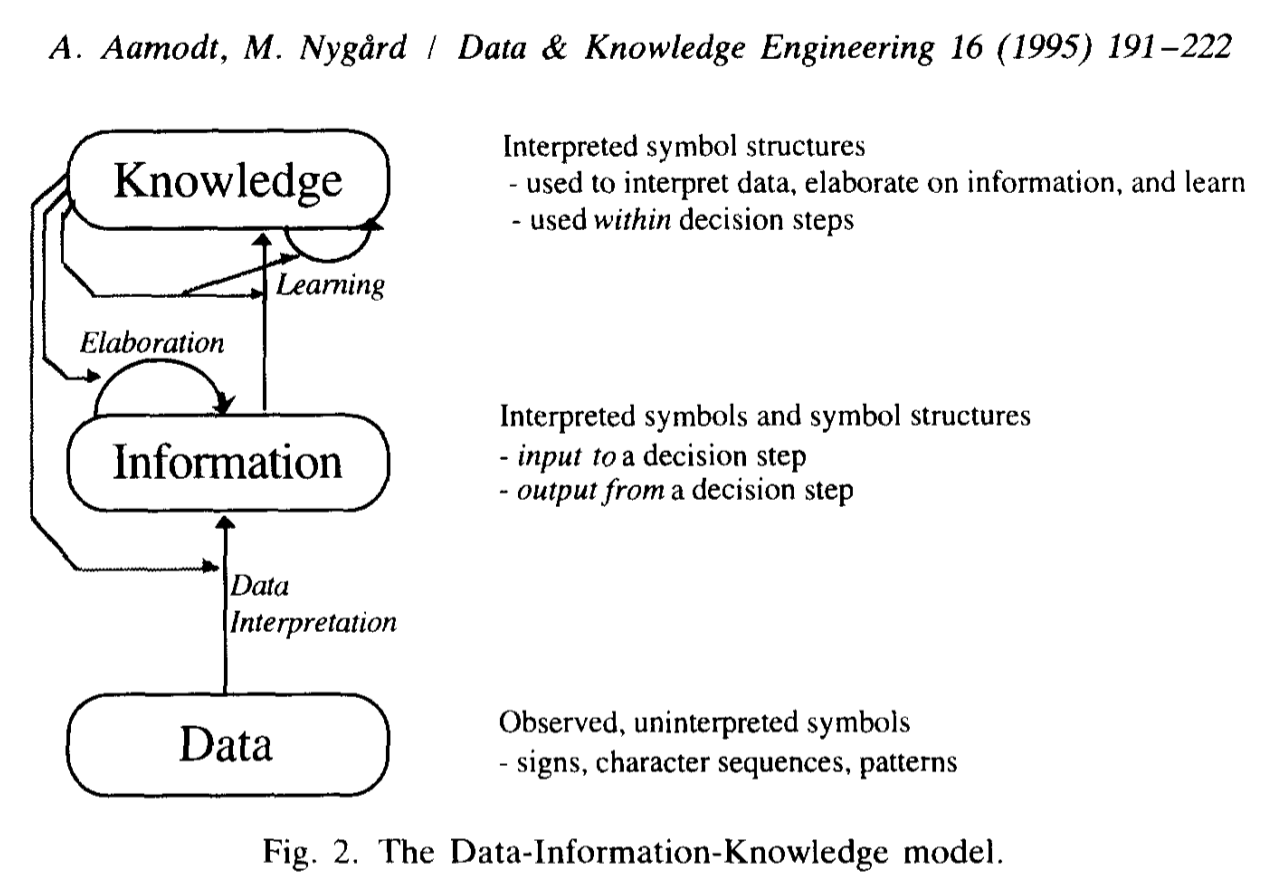
\includegraphics[scale=0.23,center]{aamodt-nygard-dik.png}
	\end{figure}	
	
	\vspace{0.1cm}
	\tiny
	\begin{flushright}
		Aamodt and Nyg{\aa}rd (1995). Different roles and mutual dependencies of data, information, and knowledge -\\An AI perspective on their integration. Data \& Knowledge Engineering, 16(3):191-222. \url{https://doi.org/10.1016/0169-023X(95)00017-M}\\
	\end{flushright}
	
\end{frame}

\begin{frame}[plain]{}
	
	\Huge
	\begin{center}
		\begin{displaymath}
		E = mc^2
		\end{displaymath}	
	\end{center}
	
\end{frame}

\begin{frame}{Floridi über Information}
	
	\begin{itemize}
		\item Luciano Floridi, Prof. Oxford Internet Institute
		\item Philosophie der Information und Informationsethik
		\item Autor von ``The Philosophy of Information'' (2013)
	\end{itemize}
	
	\begin{figure}
		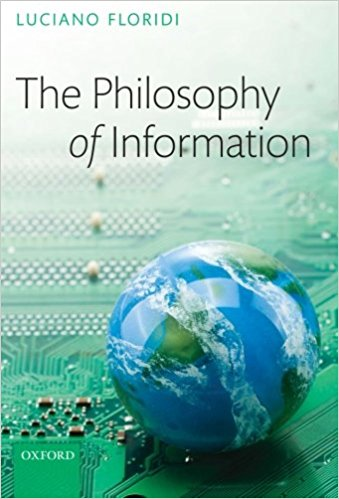
\includegraphics[scale=0.20,right]{floridi-book-cover.jpg}
	\end{figure}
	
	\tiny
	\begin{flushright}
		\url{https://global.oup.com/academic/product/the-philosophy-of-information-9780199232383}
	\end{flushright}
	
\end{frame}

\begin{frame}{Floridi über Information}
	
	\begin{itemize}
		\item Information besteht aus Daten
		\item Daten müssen wohlgeformt sein
		\item Wohlgeformte Daten müssen Bedeutungsvoll sein
		\item Wohlgeformte und Bedeutungsvolle Daten müssen wahrhaftig sein
	\end{itemize}
	
\end{frame}

\begin{frame}{Floridi über Information}
	
	\begin{itemize}
		\item Wohlgeformte und Bedeutungsvolle Daten sind semantischer Inhalt
		\item Nur wahrer semantischer Inhalt ist semantische Information
		\item Falschinformation und Desinformation keine semantische Information
	\end{itemize}
	
\end{frame}

\begin{frame}{Floridi über Information}
	
	\begin{itemize}
		\item Semantische Information unterscheidet sich von Umweltinformation
		\item Umweltinformation sind Signale der Umgebung (``natürliche Daten'')
		\item Z.B. Jahresringe, Fingerabdrücke, flüchtige organische Verbindungen
		\item Umweltinformation müss nicht zwingend Bedeutung enthalten
		\item Auch Pflanzen/Tiere können diese für praktische Zwecke nutzen
	\end{itemize}
	
\end{frame}


\begin{frame}{Information im Informationsmanagement}
	
	\begin{itemize}
		\item Informationsmanagement verwaltet Information
		\item Möglichst semantische Information
		\item Sprich wohlgeformte, bedeutungsvolle und wahrhaftige Daten
		\item Aber auch nur semantische Inhalte
		\item Es wird sicherlich auch Falschinformation verwaltet
		\item Erreichung strategischer Ziele benötigt semantische Information
	\end{itemize}
	
\end{frame}

\begin{frame}{Information im Informationsmanagement}
	
	\begin{itemize}
		\item Information wird von Informationssysteme verwaltet
		\item Die interdependenten Systeme einer Informationsinfrastruktur
		\item Insbesondere die Technik, die Soft- und Hardware des Systems
		\item Zentral für Informationsverarbeitung, -verteilung, -speicherung
	\end{itemize}
	
\end{frame}

\begin{frame}{Information im Informationsmanagement}
	
	\begin{itemize}
		\item Die Software eines Informationssystems spielt eine wichtige Rolle
		\item Diese repräsentiert, verarbeitet, verteilt, speichert Information
		\item Als wohlgeformte und bedeutungsvolle Daten
	\end{itemize}
	
\end{frame}

\begin{frame}{Wohlgeformte Daten: Die Rolle von XML}
	
	\begin{itemize}
		\item XML ist eine \emph{meta} Auszeichnungssprache
		\item Eignet sich für die Entwicklung spezifischer Auszeichnungssprachen
		\item Zur Markierung von Inhalten
		\item Wobei sich dadurch strukturierte Daten ergeben
		\item Die entsprechend den XML Sprachregeln \emph{wohlgeformt} sind
	\end{itemize}
	
\end{frame}


\begin{frame}[fragile]{Wohlgeformte Daten: Die Rolle von XML}

	Unstrukturiert
	\small\begin{lstlisting}
	Der Planet Erde hat einen Radius von 6371 km.
	\end{lstlisting}\normalsize
	
	Semistrukturiert
	\lstset{language=XML}	
	\small\begin{lstlisting}
	Der <planet>Planet <name>Erde</name> hat 
	<property>einen Radius von <radius>6371</radius> 
	<unit>km</unit></property></planet>.
	\end{lstlisting}\normalsize
	
	Strukturiert
	\lstset{language=XML}	
	\small\begin{lstlisting}	
	<planet>
	  <name>Erde</name>
	  <property>
	    <radius>6371</radius>
	    <unit>km</unit>
	  </property>
	</planet>
	\end{lstlisting}\normalsize
	
\end{frame}

\begin{frame}{Wohlgeformte Daten: Die Rolle von XML}
	
	\begin{itemize}
		\item Mit DTD / XML Schema kann man zusätzlich auf Gültigkeit prüfen
		\item Entsprechen XML Daten einem Schema, insb. Struktur, Datentypen
		\item In einem Informationssystem unterstützt XML somit die
		\begin{itemize}
			\item Repräsentation 
			\item Verarbeitung
			\item Kommunikation
			\item Speicherung
		\end{itemize}
		\item von Information, als wohlgeformte Daten
	\end{itemize}
	
\end{frame}

\begin{frame}{Wohlgeformte Daten: Die Rolle von RDF}
	
	\begin{itemize}
		\item RDF Daten sind wohlgeformt entsprechend einer RDF Syntax
		\item Informationssystem prüft Wohlgeformtheit beim Lesen und Schreiben
		\item Wie XML unterstützt auch RDF die Verwaltung von Information
		\item Insbesondere Information als wohlgeformte Daten
	\end{itemize}
	
\end{frame}

\begin{frame}{Bedeutungsvolle Daten: Die Rolle von XML}
	
	\begin{itemize}
		\item XML Daten sind ``selbstbeschreibend''
		\item Die Tags sind in der Tat meist Bedeutungsvoll
		\item Allerdings nur für Menschen eines Informationssystems
		\item Der Technik bedeutet nur die Baumstruktur etwas
		\item Und die Datentypen, da diese Interpretation von Werten einschränken
		\item Baumstruktur kann traversiert und navigiert werden (XPath)
	\end{itemize}
	
\end{frame}

\begin{frame}{Bedeutungsvolle Daten: Die Rolle von RDF}
	
	\begin{itemize}
		\item Die
		\begin{itemize}
			\item Repräsentation
			\item Verarbeitung
			\item Kommunikation
			\item Speicherung
		\end{itemize}
		\item von Information als wohlgeformte \emph{und bedeutungsvolle} Daten
		\item wird von RDF und Ontologiesprachen effektiver unterstützt
		\item Ontologien formalisieren die Bedeutung verwendeter Terminologie
		\item Gegeben sind nicht nur Symbole, z.B. \texttt{ex:Planet}, \texttt{ex:12bv}
		\item Auch deren Interpretation, ``Klasse der Dinge mit Eigenschaften ...''
		\item Wobei die spezifizierte Interpretation maschinenverarbeitbar ist
	\end{itemize}
	
\end{frame}

\begin{frame}{Interdependente Systeme: Die Rolle von XML und RDF}
	
	\begin{itemize}
		\item Die Systeme einer Informationsinfrastruktur sind interdependent
		\item Sie produzieren, konsumieren, kommunizieren Information
		\item Interdependenz beruht auf Interoperabilität
		\item Die Fähigkeit eines Systems mit anderen zusammenzuarbeiten
		\item Interoperabilität wird erhört wenn sich Systeme einigen
		\begin{itemize}
			\item Auf eine gemeinsame Syntax der ausgetauschten Daten
			\item Damit Daten auf wohlgeformtheit geprüft werden können
			\item Wie auch auf eine gemeinsame Semantik der Symbole
			\item Damit die Bedeutung der Symbole in der Infrastruktur gemeinsam ist
		\end{itemize}
		\item XML und RDF unterstützen die Interoperabilität 
		\item Konsum und Verarbeitung von Information wird vereinfacht
		\item Information als wohlgeformte und bedeutungsvolle Daten
	\end{itemize}
	
\end{frame}

\begin{frame}{XML und RDF im Informationsmanagement: Fazit}
	
	\begin{center}
		Diese Technologien unterstützen die Verwaltung von Information\\als wohlgeformte und bedeutungsvolle Daten (semantische Inhalte)\\innerhalb Informationsinfrastrukturen.
	\end{center}
	
\end{frame}

\begin{frame}[plain]{}
	
	\large
	\begin{center}
		Und zum Schluss noch dies ...	
	\end{center}
	
\end{frame}

\begin{frame}{Information in Forschungsinfrastrukturen}
	
	\begin{itemize}
		\item Informationsmanagement zentral auch in Forschungsinfrastrukturen
		\item Forschungsinfrastrukturen sind
		\begin{itemize}
			\item Einrichtungen, Ressourcen und Dienstleistungen
			\item Die speziell für wissenschaftliche Zwecke errichtet werden
			\item Und Forschung und Lehre ermöglichen oder erleichtern
		\end{itemize}
		\item Beispiele
		\begin{itemize}
			\item Laboratorien (z.B. CERN)
			\item Wissenschaftliche Grossgeräte (z.B. Large Hadron Collider)
			\item Archive, Bibliotheken, Datenbanken, Sammlungen
			\item Informationstechnische Einrichtungen
		\end{itemize}
	\end{itemize}
	
	\begin{flushright}
		\scriptsize\url{https://de.wikipedia.org/wiki/Forschungsinfrastruktur}
	\end{flushright}
	
\end{frame}

\begin{frame}{Information in Forschungsinfrastrukturen}
	
	\begin{itemize}
		\item Interpretation von Daten ist eine fundamentale Aktivität
		\item Hauptsächlich von Wissenschaftler durchgeführt
		\item Primär mittels der Technik von Informationssystemen
		\item Insbesondere in der Datenanalyse mit entsprechender Software
		\item Daten werden dabei meist in tabellarische Datenstrukturen verwaltet
		\item Diese sind somit wohlgeformt
	\end{itemize}
	
\end{frame}

\begin{frame}{Information in Forschungsinfrastrukturen: Problem}
	
	\begin{itemize}
		\item Bedeutung wird in solchen Datenstrukturen meist nicht verwaltet
		\item Die Daten sind somit wohlgeformt aber nicht bedeutungsvoll
		\item Technik eines Informationssystems verwaltet somit nicht Information
		\item Sondern nur wohlgeformte Daten
	\end{itemize}
	
\end{frame}

\begin{frame}{Projektvorschlag}
	
	\begin{itemize}
		\item Verbesserte Repräsentation der Bedeutung von Daten
		\item Wissenschaftliche Daten die in der Datenanalyse erzeugt werden
		\item Zum Beispiel numerische Zeitreihen, statistische Kennzahlen, ...
		\item Konkreter
		\begin{itemize}
			\item Entwicklung einer (bidirektionalen) Übersetzung von RDF Daten
			\item In eine Python \texttt{DataFrame} Datenstruktur
			\item Ohne Verlust an (formaler) Bedeutung der Daten
		\end{itemize}
		\item Zum Beispiel als Bachelor- oder Masterarbeit
		\item Wer dazu Lust hat oder mehr wissen möchte darf sich gerne melden!
	\end{itemize}
	
\end{frame}

\begin{frame}[fragile]{Beispiel: RDF Daten nach ...}
	
	\begin{lstlisting}
[] rdf:type sosa:Observation ;
   sosa:observedProperty :temperature ;
   sosa:hasFeatureOfInterest  :air ;
   sosa:madeBySensor :thermometer ;
   sosa:resultTime "2018-01-01T00:00:10Z"^^xsd:dateTime ;
   sosa:hasSimpleResult "3.1 degC"^^cdt:ucum .
   
[] rdf:type sosa:Observation ;
   sosa:observedProperty :temperature ;
   sosa:hasFeatureOfInterest  :air ;
   sosa:madeBySensor :thermometer ;
   sosa:resultTime "2018-01-01T00:00:20Z"^^xsd:dateTime ;
   sosa:hasSimpleResult "2.7 degC"^^cdt:ucum .
	\end{lstlisting}
	
\end{frame}

\begin{frame}[fragile]{Beispiel: ... Python \texttt{DataFrame} und wieder zurück}
	
	\begin{table}
		\begin{tabular}{|l|l|}
			\hline
			Time & Result \\
			\hline
			2018-01-01T00:00:10Z & 3.1 \\
			2018-01-01T00:00:20Z & 2.7 \\
			\hline
		\end{tabular}
	\end{table}
	
\end{frame}

\begin{frame}{Zusammenfassung}
	
	\begin{itemize}
		\item 
	\end{itemize}
	
\end{frame}

\end{document}